% Chapter 3

\chapter{Evaluation of Turbulence Models}

\label{chap:evaluation-of-turbulence-models}

Turbulence, as a phenomenon, has been notoriously difficult for a detailed physical analysis. This is further exacerbated by the seemingly endless complex interactions it gives rise to in the flow as long as any form of energy is provided.
Therefore, while modelling turbulence remains one facet of the problem, visualising and analysing the model is another equally challenging task.

As seen in the previous \chapref{chap:turbulence-modelling}, numerous Lagrangian turbulent models seem to be tested for only complex surface flows. However, a systematic analysis of isotropic turbulence problems provides greater insight into the energy spectrum and its corresponding cascade across varying length scales. A reasonable model should be able to capture the characteristic hierarchy of scales through which the energy cascade takes place. The dissipation of kinetic energy finally occurs at the scales of the order of Kolmogorov length, where the flow subsequently becomes laminar. In contrast, the injection of energy in turbulent flow generally occurs at much larger scales.

Hence, appropriate test cases must be used when analysing turbulence.

%----------------------------------------------------------------------------------------
%	Section 1 - Benchmark Problems
%----------------------------------------------------------------------------------------
\section{Benchmark Problems}
\subsection{Taylor-Green Vortex Problem}
\label{sec:taylor-green-vortex-problem}
The Taylor-Green vortex problem is a challenging case to tackle. The flow is periodic, incompressible and consists of decaying vortices.
The $2D$ case of the problem is analytically defined as given by \Eqref{eq:2d-tgv-vx} - \Eqref{eq:2d-tgv-p}.
\begin{equation}
    v_x = -U e^{bt} \cos(2\pi x) \sin(2\pi y),
    \label{eq:2d-tgv-vx}
\end{equation}
\begin{equation}
    v_y = U e^{bt} \sin(2\pi x) \cos(2\pi y),
    \label{eq:2d-tgv-vy}
\end{equation}
\begin{equation}
    p = (U e^{bt})^2 \frac{\cos(4\pi x) + \cos(4\pi y)}{4},
    \label{eq:2d-tgv-p}
\end{equation}
\begin{equation}
    b = -\frac{8\pi}{Re} \quad , \quad Re = \frac{UL}{\nu},
\end{equation}
where $(U, Re, L)$ are flow constants.

The $3D$ case of the problem, defined for a tri-periodic domain with boundary $(\Boundary = [0, 2\pi]^3)$ is initially set-up as given in \Eqref{eq:3d-tgv-vx} - \Eqref{eq:3d-tgv-vz}.
\begin{equation}
    v_{x, 0} = \sin(x) \cos(y) \cos(z),
    \label{eq:3d-tgv-vx}
\end{equation}
\begin{equation}
    v_{y, 0} = -\cos(x) \sin(y) \cos(z),
    \label{eq:3d-tgv-vy}
\end{equation}
\begin{equation}
    v_{z, 0} = 0.
    \label{eq:3d-tgv-vz}
\end{equation}
The corresponding initial pressure field $(P_0)$ obtained from solving the pressure Poisson equation for incompressible flow is given by \Eqref{eq:3d-tgv-p} \parencite{pereira2021modeling}.
\begin{equation}
    P_{0} = P_o + \frac{\rho_o \nu_o^2}{16} \bigg(2 + \cos(2z) \bigg) \bigg(\cos(2x) + \cos(2y) \bigg),
    \label{eq:3d-tgv-p}
\end{equation}

\subsection{Thin Double-Shear Layer}
The thin double-shear layer is a problem often considered to be too difficult to simulate due to the small scales which are produced. 
The main challenge of the problem, as shown by \cite{minion1997performance}, occurs when a numerical method produces spurious structures, especially when the flow is sufficiently under-resolved. 
\cite{drikakis2001spurious} studied the problem's spurious structure to understand its numerical mechanism. They indicated that the spurious structure's generation depends on the advective scheme's choice. 

The initial conditions for the $2D$ periodic flow is given by:
\begin{equation}
    v_{x, 0} = \tanh \big(80 \times \min[y-0.25, 0.75-y] \big),
    \label{eq:2d-tdsl-vx}
\end{equation}
\begin{equation}
    v_{y, 0} = \delta \sin \big( 2\pi (x+0.25) \big).
    \label{eq:2d-tdsl-vy}
\end{equation}

\subsection[3D Isotropic Turbulence]{$3D$ Isotropic Turbulence}
The JHU Turbulence Database Cluster \parencite{li2008public} provide a direct numerical simulation (DNS) data set for isotropic, forced turbulence. The data set consists of the DNS output on $1024^3$ spatial points and $1024$ time samples spanning about one large-scale turnover time.

The entire $1024^4$ space-time history of the incompressible DNS simulation $(Re\approx1460)$ is accessible to users remotely through an interface based on the Web-services model. 
The data from the database contains the three velocity components and the pressure. A uniform non-dimensionalised pressure $(P^* = \frac{P}{\rho U^2} + 1)$ is added to the
database pressure, with Mach number Ma 0.1. 

\subsection[2D Confined and Driven Turbulence]{$2D$ Confined \& Driven Turbulence}
Based on the test case employed by \cite{Monaghan2017}, a $2D$ fluid confined to a square solid impenetrable boundary is considered $(\Boundary = [0,1]^2)$. A cylinder of radius $(r=0.7)$ is placed at the centre of the box. The circle is subsequently provided with a Lissajous trajectory to follow given by \Eqref{eq:2d-cdt-x} - \Eqref{eq:2d-cdt-y}.
\begin{equation}
    x = 0.5 + 0.25 \sin \bigg( \frac{2\pi t}{5} \bigg)
    \label{eq:2d-cdt-x}
\end{equation}
\begin{equation}
    y = 0.5 + 0.25 \sin \bigg( \frac{4\pi t}{5} \bigg)
    \label{eq:2d-cdt-y}
\end{equation}

\subsection{Free Surface Flows}
As seen in numerous works involving turbulence models in the previous chapter, there does not appear to be any dearth of experimental and numerical research on free-surface flows. Problems ranging from the classic $2D$ and $3D$ dam break to wave propagation, wave breaking, water overtopping, and dyke-flow inspired problems can be simulated. The only caveat involved in such cases includes the resolution requirements of the problem and the approach taken in free surfaces boundary condition implementation.

%----------------------------------------------------------------------------------------
%	Section 2 - Post-Simulation Analysis
%----------------------------------------------------------------------------------------
\section{Post-Simulation Analysis}
\subsection{Energy Spectral Density}
In order to analyse the predicted flow and validate the turbulent model, energy spectra are the most used description since it has to fall off as prescribed by the  Kolmogorov - $5/3$ Law.
Typical mesh or grid-based methods facilitate the calculation of the energy spectrum $(E[\WaveNumber])$ by using the Fourier transform of the velocity field as given in \Eqref{eq:Shi2013-vel-FT}, to obtain the velocity spectrum as defined in \Eqref{eq:Shi2013-vel-spectrum}.
\begin{equation}
    \vect{V}(\vect{k}) = \frac{1}{L^3} \int \exp(-i \vect{k} \cdot \vect{r}) \vect{v}(\vect{r}) d\vect{r}
    \label{eq:Shi2013-vel-FT}
\end{equation}
Where $(d\vect{r}=dxdy)$ for $2D$ and $(d\vect{r}=dxdydz)$ for $3D$, and $[\vect{k} = (\WaveNumber_x, \WaveNumber_y, \WaveNumber_z)]$ is the wave-number vector.
\begin{equation}
    E(\vect{k}) = \HalfFrac \abs{ \vect{V}(\vect{k}) \cdot \vect{V}^*(\vect{k}) }
    \label{eq:Shi2013-vel-spectrum}
\end{equation}

The energy spectrum is subsequently defined as given by \Eqref{eq:Shi2013-energy-spectrum} for the case of isotropic turbulence.
\begin{equation}
    E(\WaveNumber) = B \langle E(\vect{k}) \rangle \quad , \quad \WaveNumber = \abs{\vect{k}}
    \label{eq:Shi2013-energy-spectrum}
\end{equation}
Where $(B=2\pi k)$ for $2D$ and $(B=4\pi k^2)$ for $3D$.

However, SPH does not have such grid-like data to calculate the energy spectrum directly. Hence, the data has to be reconstructed using interpolation methods as outlined by \cite{Shi2013}.
The authors provide three distinct methods of interpolating the data across a grid-like space. 
The SPH interpolation method specified by the authors is given in \Eqref{eq:Shi2013-sph-interpolation}.
\begin{equation}
    A(\vect{r}) \approx \sum_j A_j W(\abs{\vect{r} - \vect{r}_j}, h) \Vol_j
    \label{eq:Shi2013-sph-interpolation}
\end{equation}

The remeshed interpolation method is outlined in \Eqref{eq:Shi2013-remeshed-interpolation}.
Remeshed Interpolation
\begin{equation}
    A(\vect{r}) \approx \sum_j A_j \Tilde{W}(\abs{x-x_j}, h) \Tilde{W}(\abs{y-y_j}, h) \Tilde{W}(\abs{z-z_j}, h)
    \label{eq:Shi2013-remeshed-interpolation}
\end{equation}
Where $(\Tilde{W})$ represents the kernel where the volume of the particle $(\Vol_j)$ has been absorbed.

The authors also detail the moving least squares (MLS) method as an interpolation tool. Building on the work of \cite{lancaster1981surfaces}, who were able to extend the $2D$ interpolation technique proposed by \cite{shepard1968two} to a general higher-order case. The authors state that they start with a weighted least squares formulation for an arbitrary fixed point and then move said point across the entire domain. This allows for the computation of a weighted least squares fit function, which can be used to evaluate grid-like points.

\subsection{Lagrangian Coherent Structures}
Complex flow cannot only be analysed through primitive flow properties such as pressure, velocity or energy density for a deep understanding of the flow interactions. Techniques using only such properties would fail to identify general coherent structures (CS) in the flow. To facilitate that, quantities such as those employing the velocity gradient, such as the vorticity, Q-criterion, $\Delta$-criterion, swirling strength criterion, etc., are used. 
However, \cite{haller2005objective} was able to show that in some situations, most of the definitions of the vortex are not objective and suitable for studying the flow, particularly in the context of $3D$ flow.

Therefore, \cite{sun2016detection} utilise the Lagrangian Coherent Structures (LCSs) as an alternative way with specific advantages for drawing the CSs from a given flow field. In order to identify the LCSs with an objective quantity, the authors use the Finite-time Lyapunov Exponent (FTLE), which represents the rate of separation of the nearby fluid particles over a finite time interval. FTLEs can be evaluated both in forward and backward time directions.

The authors summarise the main advantages of FTLEs over different velocity gradient-based metrics as follows:
\begin{itemize}
    \item Local fluctuations of the velocity field do not induce noise to FTLEs since they are integrated in time.
    
    \item FTLE is formulated in the Lagrangian frameworks allowing for better identification of the LCSs with respect to quantities derived from the velocity gradient.
    
    \item FTLE can identify LCSs with an accuracy that, in some cases, resemble those obtained from advanced experimental techniques.
\end{itemize}

\begin{figure}[htbp!]
    \centering
    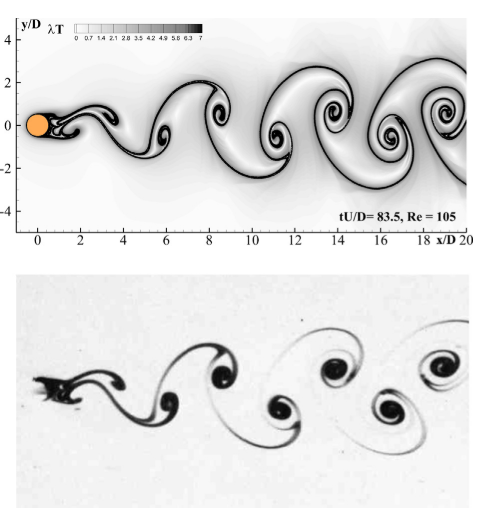
\includegraphics{Figures/research_papers/sun2016detection-fig-1.png}
    \caption{Viscous flow past a circular cylinder at $Re = 105$. Top: Attracting FTLE contour plot from SPH simulation. Bottom: Photo from experiments conducted by \cite{taneda1977visual} with electrolytic precipitation in water technique for vortex street visualisation. Reproduced from \cite{sun2016detection}}
    \label{fig:sun2016detection-fig-1}
\end{figure}

The forward-in-time FTLE is calculated using the forward-in-time Right-Cauchy–Green strain tensor, while backward-in-time FTLE requires the Left-Cauchy–Green strain tensor.
The authors propose two methods to calculate a flow's Cauchy–Green strain tensors.

The first method uses SPH formulations for the deformation gradient to compute the Cauchy–Green strain tensors. The backward-in-time FTLE can be computed using limited resources during run-time concurrently in this method. However, the forward-in-time FTLE can only be computed during post-processing.

In the second method, the forward-in-time deformation gradient is evolved as a property within the simulation's time integration step employing a governing equation for the property. This method does not need to keep track of the spatial relation between the points. This allows for the process to be suitable for Eulerian solvers as well.
Building on this work, \cite{dauch2018highly} developed an efficient GPU-based implementation to accelerate the computation of FTLE fields or, depending on the architecture of the solver, completely move the step from being calculated on the CPU to the GPU. Their proposition is highly enticing, especially for $3D$ flows.

% TODO: More details of Sun2016 required